\documentclass[UTF8,a4paper,10pt,nocolorlinks]{ctexart}
\usepackage[left=2.50cm, right=2.50cm, top=2.50cm, bottom=2.50cm]{geometry} %页边距
\CTEXsetup[format={\Large\bfseries}]{section} %设置章标题居左   
\usepackage{ctex}
\CTEXoptions[today=old]
\usepackage{cite}
% 代码块儿
\usepackage{textcomp} % 必须加上,否则报错
\usepackage{listings}
\usepackage{xcolor}
% \usepackage{fontspec}
% \setmonofont{Consolas}
\usepackage{varioref}       % ref 跨页调用
\usepackage{ctex}
\usepackage{multicol}
\usepackage{amssymb}        % 等于号 上面 加一个三角形
\usepackage{setspace}
\usepackage{tikz} % package used for the tikz
\usepackage{mdframed}
\usepackage{titletoc}
\usepackage{etoolbox}

\usepackage{helvet}
\usepackage{caption}
\usepackage{multicol} %用于实现在同一页中实现不同的分栏
\usepackage{changepage}
\usepackage{graphics}
\usepackage{amsmath, amsfonts, amssymb} % math equations, symbols
\usepackage[english]{babel}
\usepackage{color}      % color content 设置字体颜色
\usepackage{graphicx}   % import figures
\usepackage{url}        % hyperlinks
\usepackage{bm}         % bold type for equations
\usepackage{multirow}
\usepackage{booktabs}
\usepackage{epstopdf}
\usepackage{epsfig}
\usepackage{algorithm}
\usepackage{algorithmic}

\usepackage[pagestyles]{titlesec}
% \renewcommand{\algorithmicrequire}{ \textbf{Input:}}     % use Input in the format of Algorithm  
% \renewcommand{\algorithmicinput}{ \textbf{Input:}}     % use Input in the format of Algorithm  
\renewcommand{\algorithmicensure}{ \textbf{Input:}} % use Initialize in the format of Algorithm  
% \renewcommand{\algorithmicreturn}{ \textbf{Output:}}     % use Output in the format of Algorithm  
\renewcommand{\figurename}{图}
% 引用参考文献标号显示在右上角
\newcommand{\upcite}[1]{\textsuperscript{\textsuperscript{\cite{#1}}}}

\newpagestyle{teststyle}{
  \sethead{学号: 2019520941}{\sectiontitle}{第\thepage页}
  \renewcommand{\makeheadrule}{
    \makebox[0pt][l]{\rule[-.3\baselineskip]{\linewidth}{.5pt}}
    \rule[-.4\baselineskip]{\linewidth}{.5pt}
  }
}
\usepackage{color}
\usepackage{subfigure}
\usepackage{changepage}
\usepackage{fancyhdr} %设置页眉、页脚
\pagestyle{fancy}  %%%单线页眉
\fancyhead{}
\fancyhead[LO]{chapter 3 notebook}
\fancyhead[RO]{fengxuewei}
% \fancyfoot[RO]{\thepage}
\fancypagestyle{plain}{%
  \pagestyle{fancy}
}
\usepackage{shorttoc}
\usepackage{xcolor}
\usepackage{mdframed}
\usepackage{titletoc}
% \renewcommand{\today}{\CJKnumber\year 年 \CJKnumber\month 月 \CJKnumber\day 日}

\DeclareRobustCommand{\chuhao}{\fontsize{42pt}{\baselineskip}\selectfont}  % 初号
\DeclareRobustCommand{\xiaochu}{\fontsize{36pt}{\baselineskip}\selectfont} % 小初
\DeclareRobustCommand{\yihao}{\fontsize{26pt}{\baselineskip}\selectfont}   % 一号
\DeclareRobustCommand{\xiaoyi}{\fontsize{24pt}{\baselineskip}\selectfont}  % 小一
\DeclareRobustCommand{\erhao}{\fontsize{22pt}{\baselineskip}\selectfont}   % 二号
\DeclareRobustCommand{\xiaoer}{\fontsize{18pt}{\baselineskip}\selectfont}  % 小二
\DeclareRobustCommand{\sanhao}{\fontsize{16pt}{\baselineskip}\selectfont}  % 三号 
\DeclareRobustCommand{\xiaosan}{\fontsize{15pt}{\baselineskip}\selectfont} % 小三
\DeclareRobustCommand{\sihao}{\fontsize{14pt}{\baselineskip}\selectfont}   % 四号
\DeclareRobustCommand{\xiaosi}{\fontsize{12pt}{\baselineskip}\selectfont}  % 小四
\DeclareRobustCommand{\wuhao}{\fontsize{10.5pt}{\baselineskip}\selectfont} % 五号
\DeclareRobustCommand{\xiaowu}{\fontsize{9pt}{\baselineskip}\selectfont}   % 小五
\DeclareRobustCommand{\liuhao}{\fontsize{7.5pt}{\baselineskip}\selectfont} % 六号
\DeclareRobustCommand{\xiaoliu}{\fontsize{6.5pt}{\baselineskip}\selectfont}% 小六
\DeclareRobustCommand{\qihao}{\fontsize{5.5pt}{\baselineskip}\selectfont}  % 七号

\lstset{numbers=left,numberstyle=\tiny,
breaklines=true,  %代码过长则换行
keywordstyle=\color{blue!70},commentstyle=\color{red!50!green!50!blue!50},frame=shadowbox, rulesepcolor=\color{gray!20!green!20!blue!20},escapeinside=``,xleftmargin=2em,xrightmargin=2em, aboveskip=1em}

\providecommand{\keywords}[1]{\textbf{\textit{keywords---}} #1}

 
\usepackage{hyperref} %bookmarks
% \usepackage[colorlinks,linkcolor=red,anchorcolor=blue,citecolor=green,CJKbookmarks=True]{hyperref}
\hypersetup{colorlinks, bookmarks, unicode} % unicode
 
\captionsetup[figure]{labelfont={bf},labelformat={default},labelsep=period,name={图}}
\newenvironment{figurehere}
{\def\@captype{figure}}
{}
 
% \title{\textbf{A*算法和模拟退火算法无人机领域的应用}}
% \author{ 冯学伟 \thanks{学号:2019520941}}
% \date{\today}

%标题、作者及日期
% \huge{\textbf{无人机导航控制}}\\[3mm]
% \Large{\textbf{The Navigational Control In The Field Of Unmanned Air Vehicle}}\\[1mm]

\title{chapter 3. Kinematics and Dynamics}
\author{冯学伟}
\date{\today}

\begin{document}
    \maketitle
		The first step in developing navigation, guidance, and control strategies (策略) for MAVs is to develop appropriate dynamic models. Deriving the nonlinear equations of motion for a MAV is the focus of chapters 3 and 4. In chapter 5, we linearize the equations of motion to create transfer-function and state-space models(状态空间模型) appropriate 适当的 for control design. 
    第三章和第四章 推导 非线性动力学方程
第五章线性动力学方程 创建传递函数和状态空间模型 \par
	In this chapter, we derive the expressions for the kinematics 动力学 and the dynamics of a rigid body(刚体). We will apply Newton’s laws 牛顿定律: for example,
$f = m \dot{v}$ in the case of the linear motion. In this chapter, we will focus on defining the relations between positions and velocities (the kinematics) and relations between forces and moments and the momentum (dynamics). 
第三章, 定义位置和速度的关系和力与时刻和动力学的关系. 
In chapter 4, we will concentrate on the definition of the
forces and moments involved, particularly the aerodynamic forces and moments. 
第四章, 力和时刻的定义, 尤其是空气动力和时刻. 
In chapter 5, we will combine these relations to form the complete nonlinear equations of motion. 
第五章, 合并上面关系, 来形成复杂的非线性动力学方程. 
While 然而 the expressions derived in this chapter are general to any rigid body, we will use notation 符号 and coordinate frames that are typical in the aeronautics literature 航空专业领域内. In
particular, in section 3.1 we define the notation that will be used for MAV state variables MAV的状态变量的声明. In section 3.2 we derive the kinematics 推导出运动学 , and in
section 3.3 we derive the dynamics 推导出动力学方程.
\par 补充: 
Kinematics and dynamics are branches of mechanics, which is the study of forces and motion in physics.\par
Kinematics is the study of motion of particles 粒子 and bodies 物体, without taking into account the factors that cause motion 而不考虑引起运动的因素。Kinematics takes into account quantities 考虑量 such as displacement 位移, velocity, acceleration.\par
Dynamics is the study of motion, along with 连同 一起  the factors that cause motion. Calculations in dynamics, therefore, involve masses and forces. Consequently 所以, study of quantities such as momenta 瞬间 can be considered as a part of dynamics.\par
Kinematics: 	着重于结果, 不考虑原因和过程; \par
Dynamics: 		原因加结果, 并且计算动力学方程;
\par
\section{state variables 状态变量}

In developing the equations of motion for a MAV, 
twelve 十二 state variables will be introduced. 
(引入十二个状态变量: 
和平移运动相关的三个位置变量; 三个速度变量;
和旋转运动有关的三个角度变量; 三个角速度变量.
).
There are three position states and three velocity
states associated with the translational 平移的 motion 
of the MAV. Similarly,
there are three angular position and three angular velocity
states associated with the rotational motion. The state variables are listed in
\par 
\begin{itemize}
  \item The vehicle frame (NED,原点是在 机体的质心) , 绕z轴($k^{v}$)旋转chi 角度得到yaw, 即the vehicle-1 frame
  \item The vehicle-1 frame (NED,原点是在 机体的质心) , 绕y轴($j^{v1}$)旋转theta 角度得到pitch, 即the vehicle-2 frame
  \item The vehicle-2 frame (NED,原点是在 机体的质心) , 绕x轴($i^{v2}$)旋转phi 角度得到roll , 即the body frame
  \item $i^{b}$被指向飞机的机头
  \item $j^{b}$被指向飞机的右翼
  \item $K^{b}$被指向飞机的肚皮belly 
  \item vehicle-2 frame:  
  \item $i^{v2}$被指向飞机的机头
  \item $j^{v2}$被指向飞机的右翼
  \item $K^{v2}$被指向飞机的肚皮belly
  \item $u$ : 体坐标系下的$i^{b}$上的速度
  \item $v$ : 体坐标系下的$j^{b}$上的速度
  \item $\omega$ : 体坐标系下的$k^{b}$上的速度
  \item $\phi$ : roll ($F^{v2}$)
  \item $\theta$ : pitch ($F^{v1}$)
  \item $\psi$ : yaw ($F^{v}$)
  \item $p$ roll rate (体坐标系下)
  \item $q$ pitch rate (体坐标系下)
  \item $r$ yaw rate (体坐标系下)
  \label{table_3}
\end{itemize}

Because the Euler angles are defined relative to intermediate 中间的 frames of reference, we cannot say that the angular rates ($p$, $q$, $r$) are simply the time derivatives of the attitude angles ($\phi, \theta, \psi$).
. 因为欧拉角是定义为中间的坐标系(vehicle-2 / 1)不能说 角速率是姿态角相对于时间的导数.\par
下面章节中我们看到的 $p = \dot{\phi}, q = \dot{\theta}, r = \dot{\psi}$ 仅仅在 $\phi = \theta = 0$ 的时候成立. \par
\textcolor{red}{本章的其余部分专门用于制定与\ref{table_3}中列出的每个状态相对应的运动方程式}.

\section{Kinematics}
The translational 位移的 velocity of the MAV is commonly expressed in terms
of the velocity components along each of the axes in a body-fixed
coordinate frame. The components $u, v$, and $w$ correspond to the
inertial velocity of the vehicle projected onto the $i^{b}, j^{b}, and k^{b}$ axes,
respectively. On the other hand, the translational position of the MAV is
usually measured and expressed in an inertial reference frame. Relating
the translational velocity and position requires differentiation 微分 and a
rotational transformation 旋转变形, 见公式\ref{equ_1}
\begin{figure}[htpb]
  \centering
  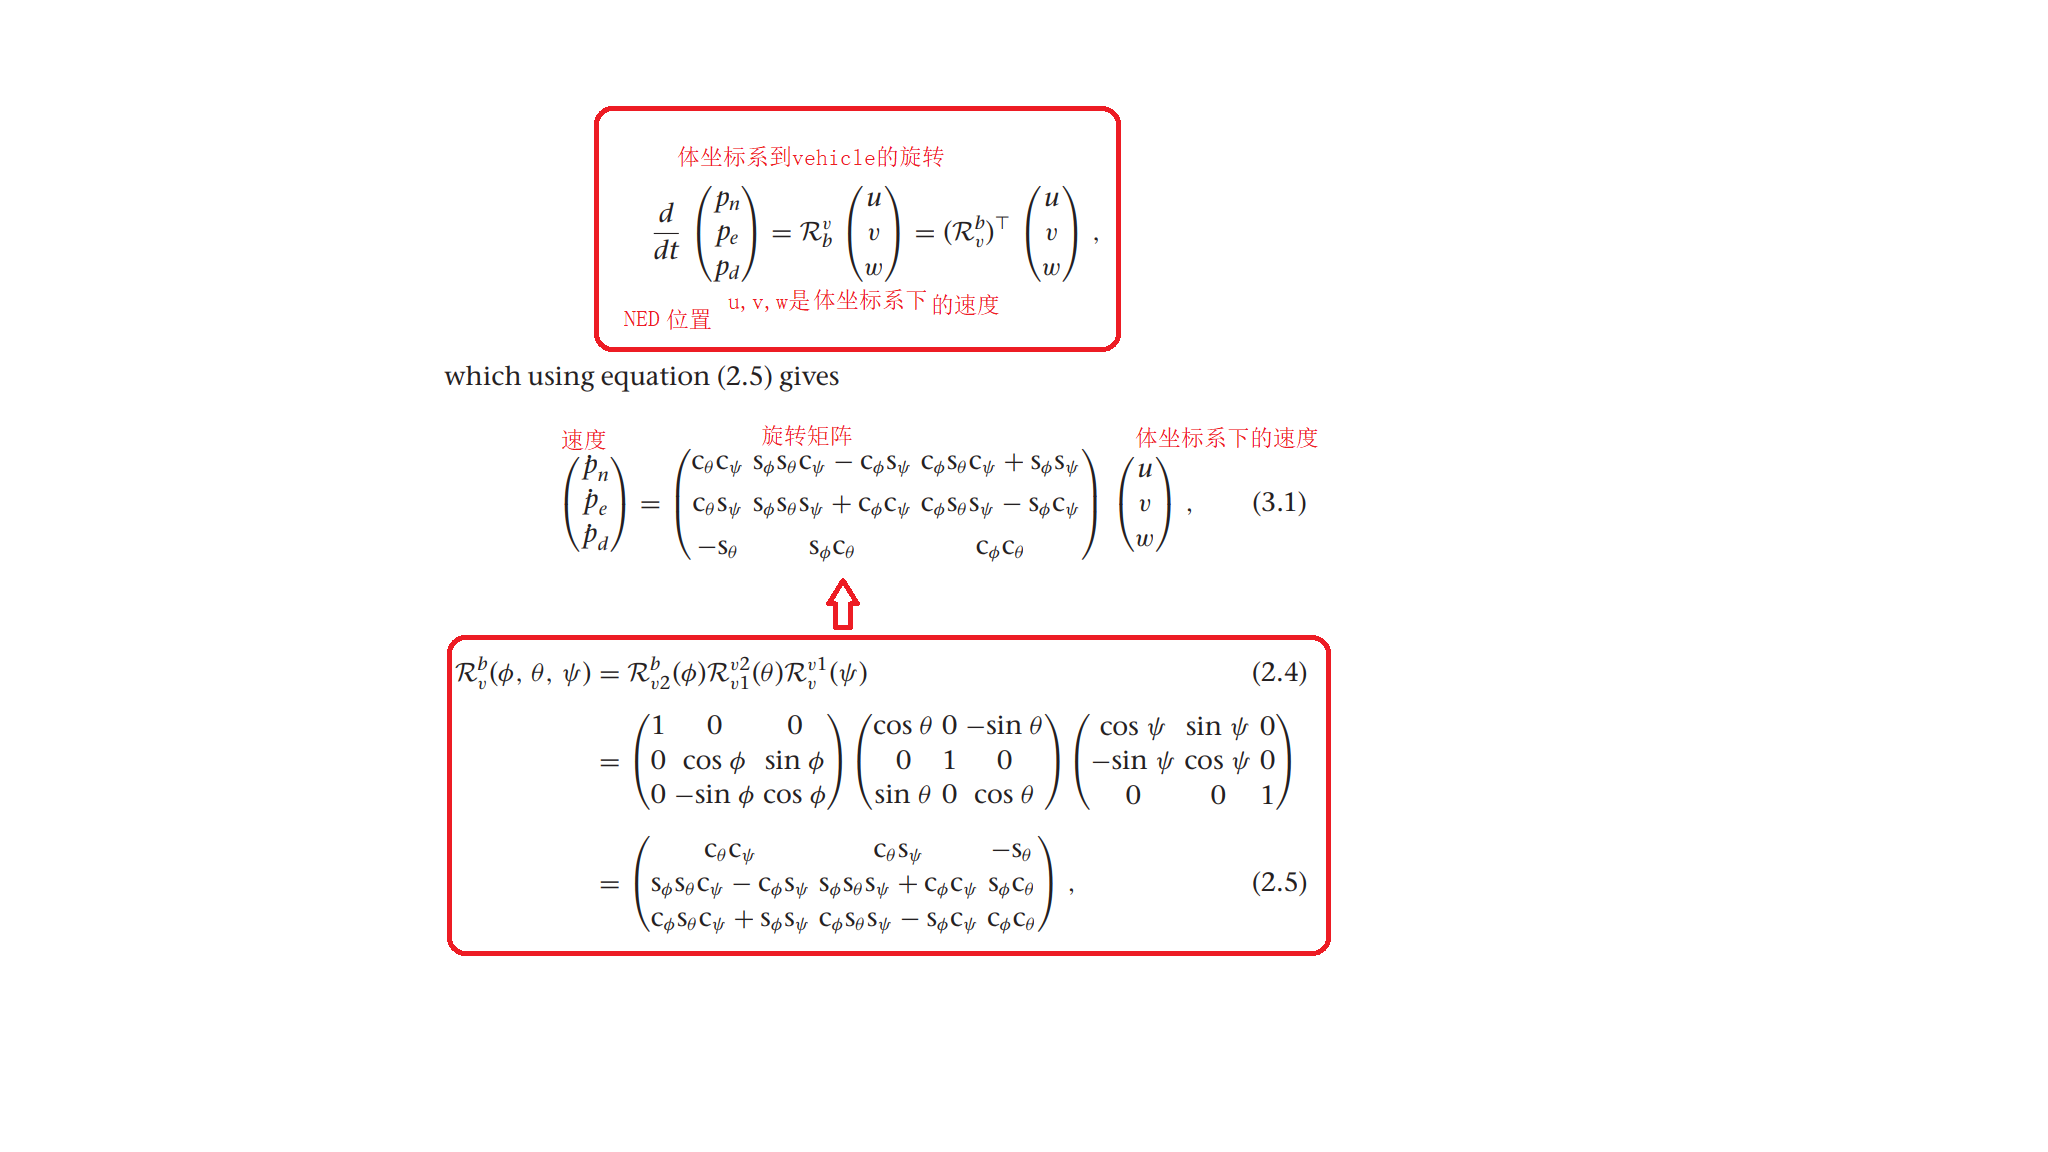
\includegraphics[width=\textwidth]{picture/equ_1.png}
  \caption{NED下的位置导数}
  \label{equ_1}
\end{figure}

\par 欧拉角$\phi, \theta, \psi$ (坐标系Vehicle, Vehicle-1, Vehicle-2)和角速率 $p, q, r$(体坐标) 因被定义在不同的坐标系下而复杂, (yaw, pitch, roll 对应着 vehicle到vehicle-1(k轴), vehicle-1到vehicle-2(j轴), vehicle-2到body(i轴))
, 将它们分别从各自的坐标系旋转变换到body坐标系进行求速率, 继而求和即可 \ref{equ_2}

\begin{figure}[htpb]
  \centering
  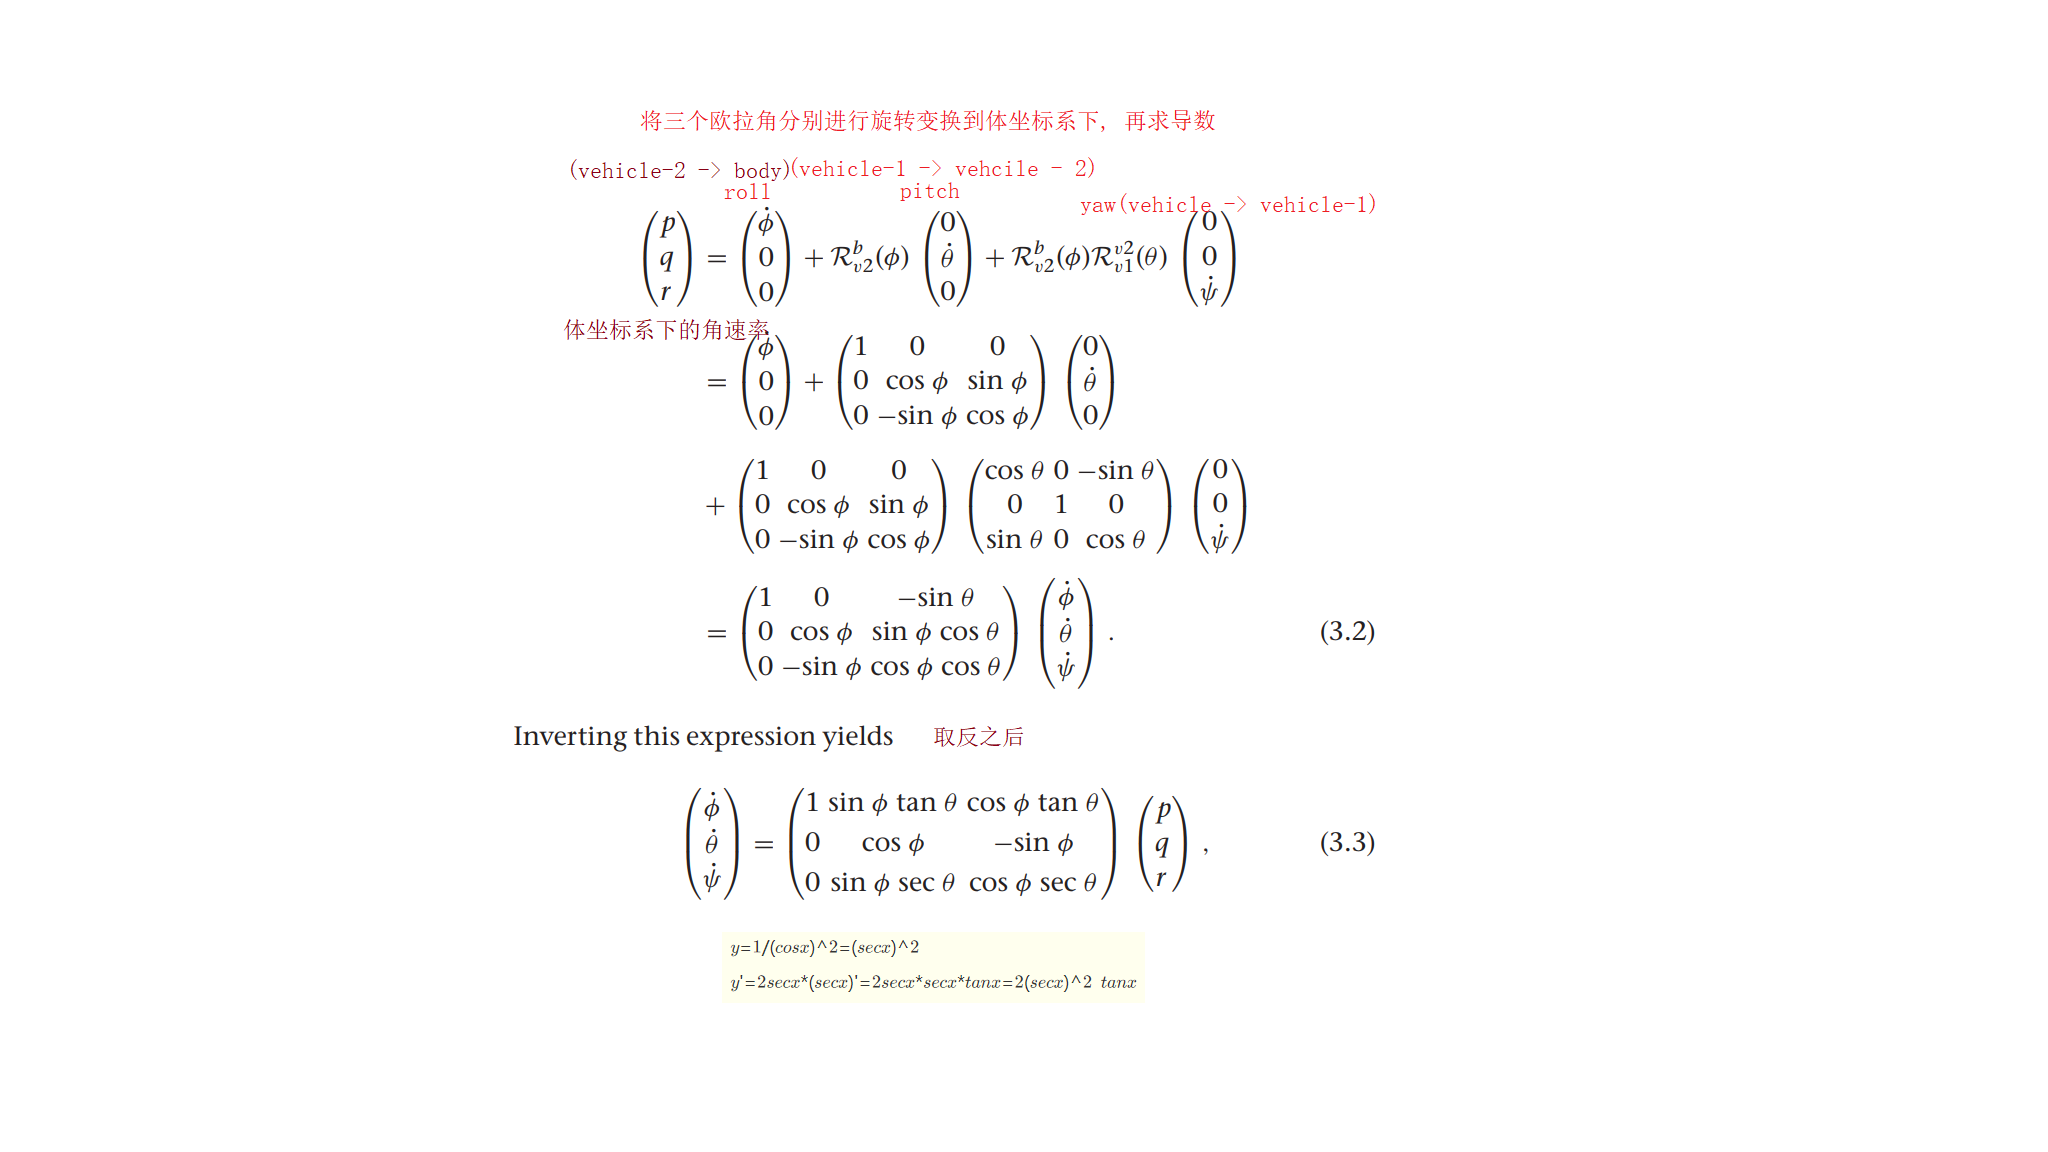
\includegraphics[width=\textwidth]{picture/equ_2.png}
  \caption{旋转坐标系, 继而求和, 得到体坐标系下的角速率}
  \label{equ_2}
\end{figure}

\section{Rigid-body Dynamics}
\subsection{Newton's second law}
牛顿第二运动定律的常见表述是:(作用在 惯性坐标系 , 即物体的运动被固定在一个固定的坐标系下, 这里是大地坐标系(ground), 尽管如此, 我们也是可以使用向量(和其他的坐标系所联系的向量)来进行表示)
\begin{equation}
  F = ma \nonumber
\end{equation}
\begin{itemize}
  \item 物体加速度的大小跟作用力成正比,跟物体的质量成反比,
  \item 且与物体质量的倒数成正比;加速度的方向跟作用力的方向相同。
\end{itemize}
\subsection{向量的微分}
向量的叉乘(a x b) = 在数值上等于由向量a和向量b构成的平行四边形的面积, 公式推导可见\ref{2_equ}
\begin{figure}[htpb]
  \centering
  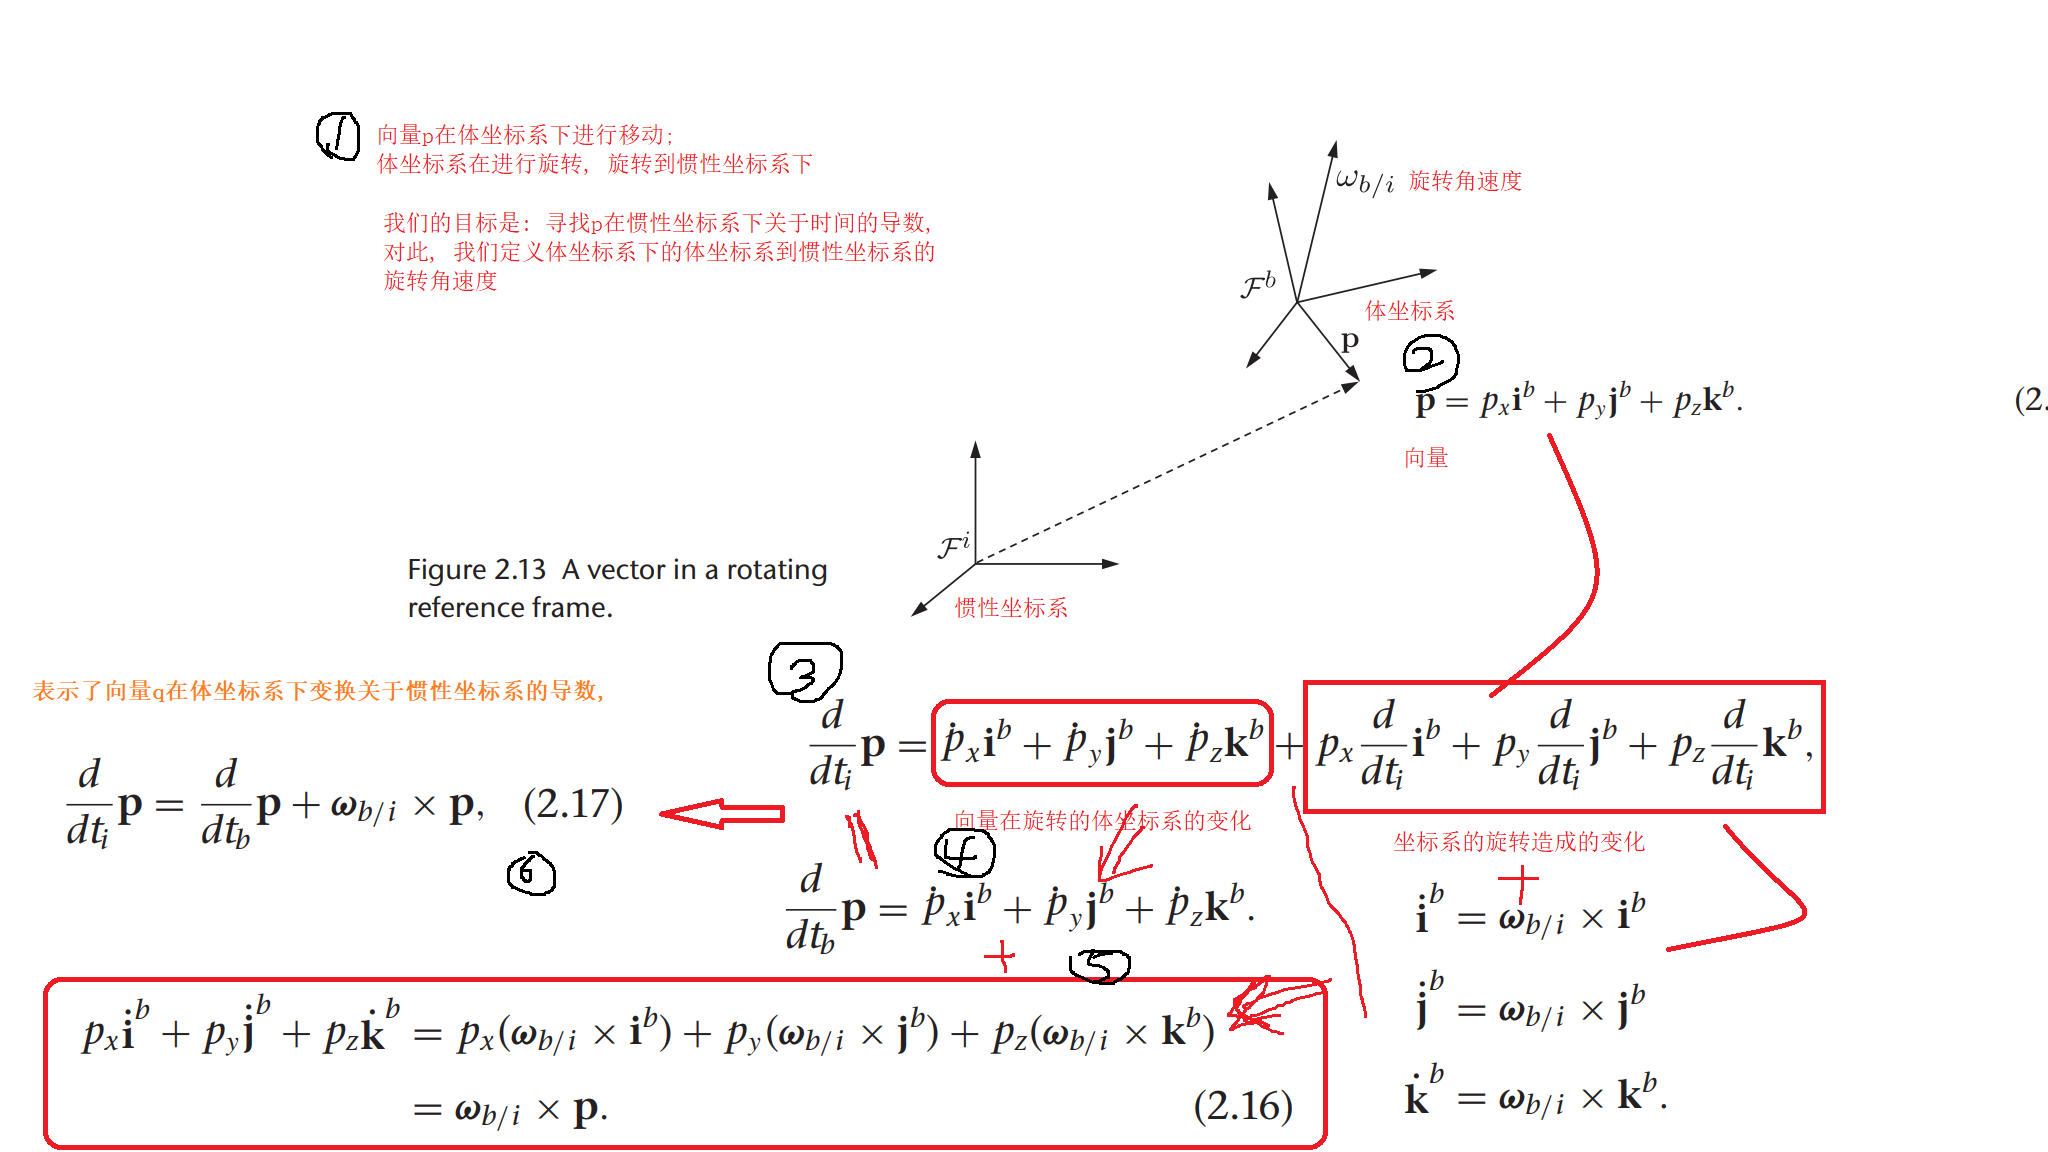
\includegraphics[width=0.8\textwidth]{picture/2_equ.png}
  \caption{向量的微分}
  \label{2_equ}
\end{figure}
\subsection{向量的叉积}
见\ref{equ_4}
\begin{figure}[htpb]
  \centering
  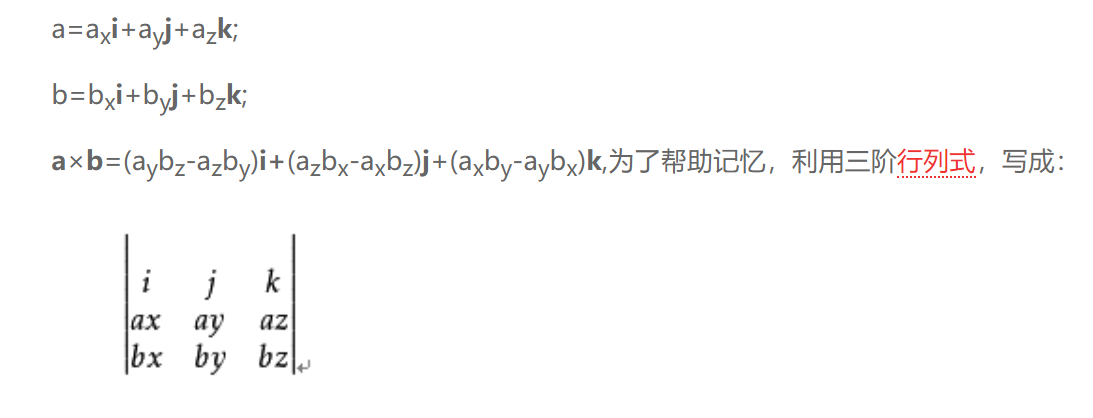
\includegraphics[width=0.8\textwidth]{picture/crossProduct.png}
  \caption{叉积计算}
  \label{equ_4}
\end{figure}
\subsection{叉乘矩阵}
见: \ref{equ_cproduct}
\begin{figure}[htpb]
  \centering
  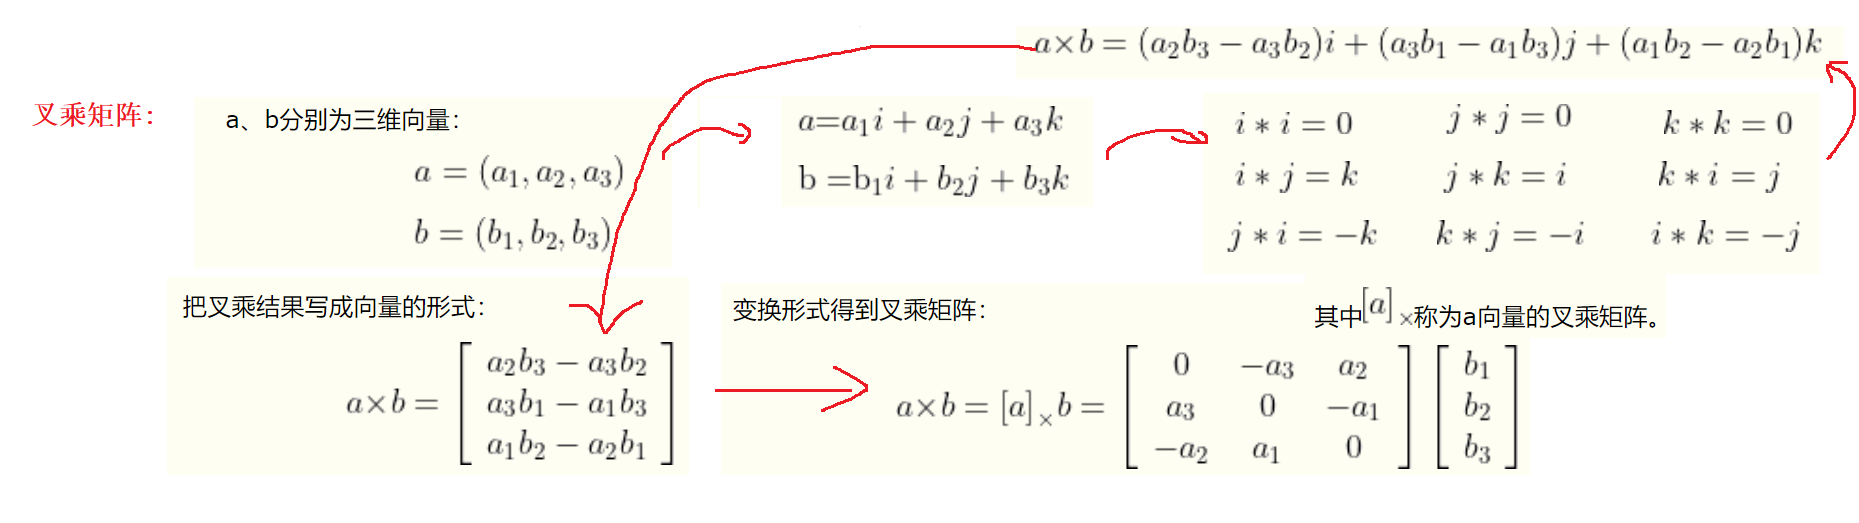
\includegraphics[width=0.8\textwidth]{picture/cproductMat.png}
  \caption{叉乘矩阵}
  \label{equ_cproduct}
\end{figure}

\section{转动惯量}
定义: 刚体绕轴转动时惯性的量度, 用字母$I$或$J$表示
\par 公式:
\begin{equation}
  I = m * r^{2} \nonumber
\end{equation}
其中的m是物体的质量, r是质点和转轴的垂直距离. 单位是 $kg \dot m^{2}$
\section{角动量}
定义: 物体在转动的时候, 具有的"冲动".
\par 公式: 
\begin{equation}
  L = velocity * radius * mass
\end{equation}
其中, velocity是速度, radius是转弯的半径, mass是物体的质量.

\par 系统的角动量守恒定律: 
一个系统内的所有物体的旋转运动所具有的角动量之和是不会随着时间的变化而变化的. 除非有外界因素的干扰. 
\section{力矩}
定义: 力矩表示力对物体作用时所产生的转动效应的物理量。 力矩是产生转动效应的原因. 
\par 公式: 
\begin{equation}
  \textbf{M} = \textbf{L} \times \textbf{F}
\end{equation}
其中的 L 是转动轴到着力点的距离矢量, F是矢量力. 力矩也是一个矢量. 


\subsection{Rigid-body Dynamics}
first to the translational degrees of freedom and then to the rotational degrees of freedom.
首先平移自由度, 然后旋转自由度.\\
假设: 平缓的地面模型, 对于小型无人机是适用的. \\
MAV的速度向量是$V_{g}$, 这个变量是方便的对于大多数体坐标系下的公式表达, 体坐标系下的速度向量为 $V_{g}^{b} = (u, v, w)$. 

\clearpage
\subsection{translational motion}
针对无人机做平移运动, 牛顿第二定律作用在物体上面的动力学模型 \ref{equ_3}. 
\begin{figure}[htpb]
  \centering
  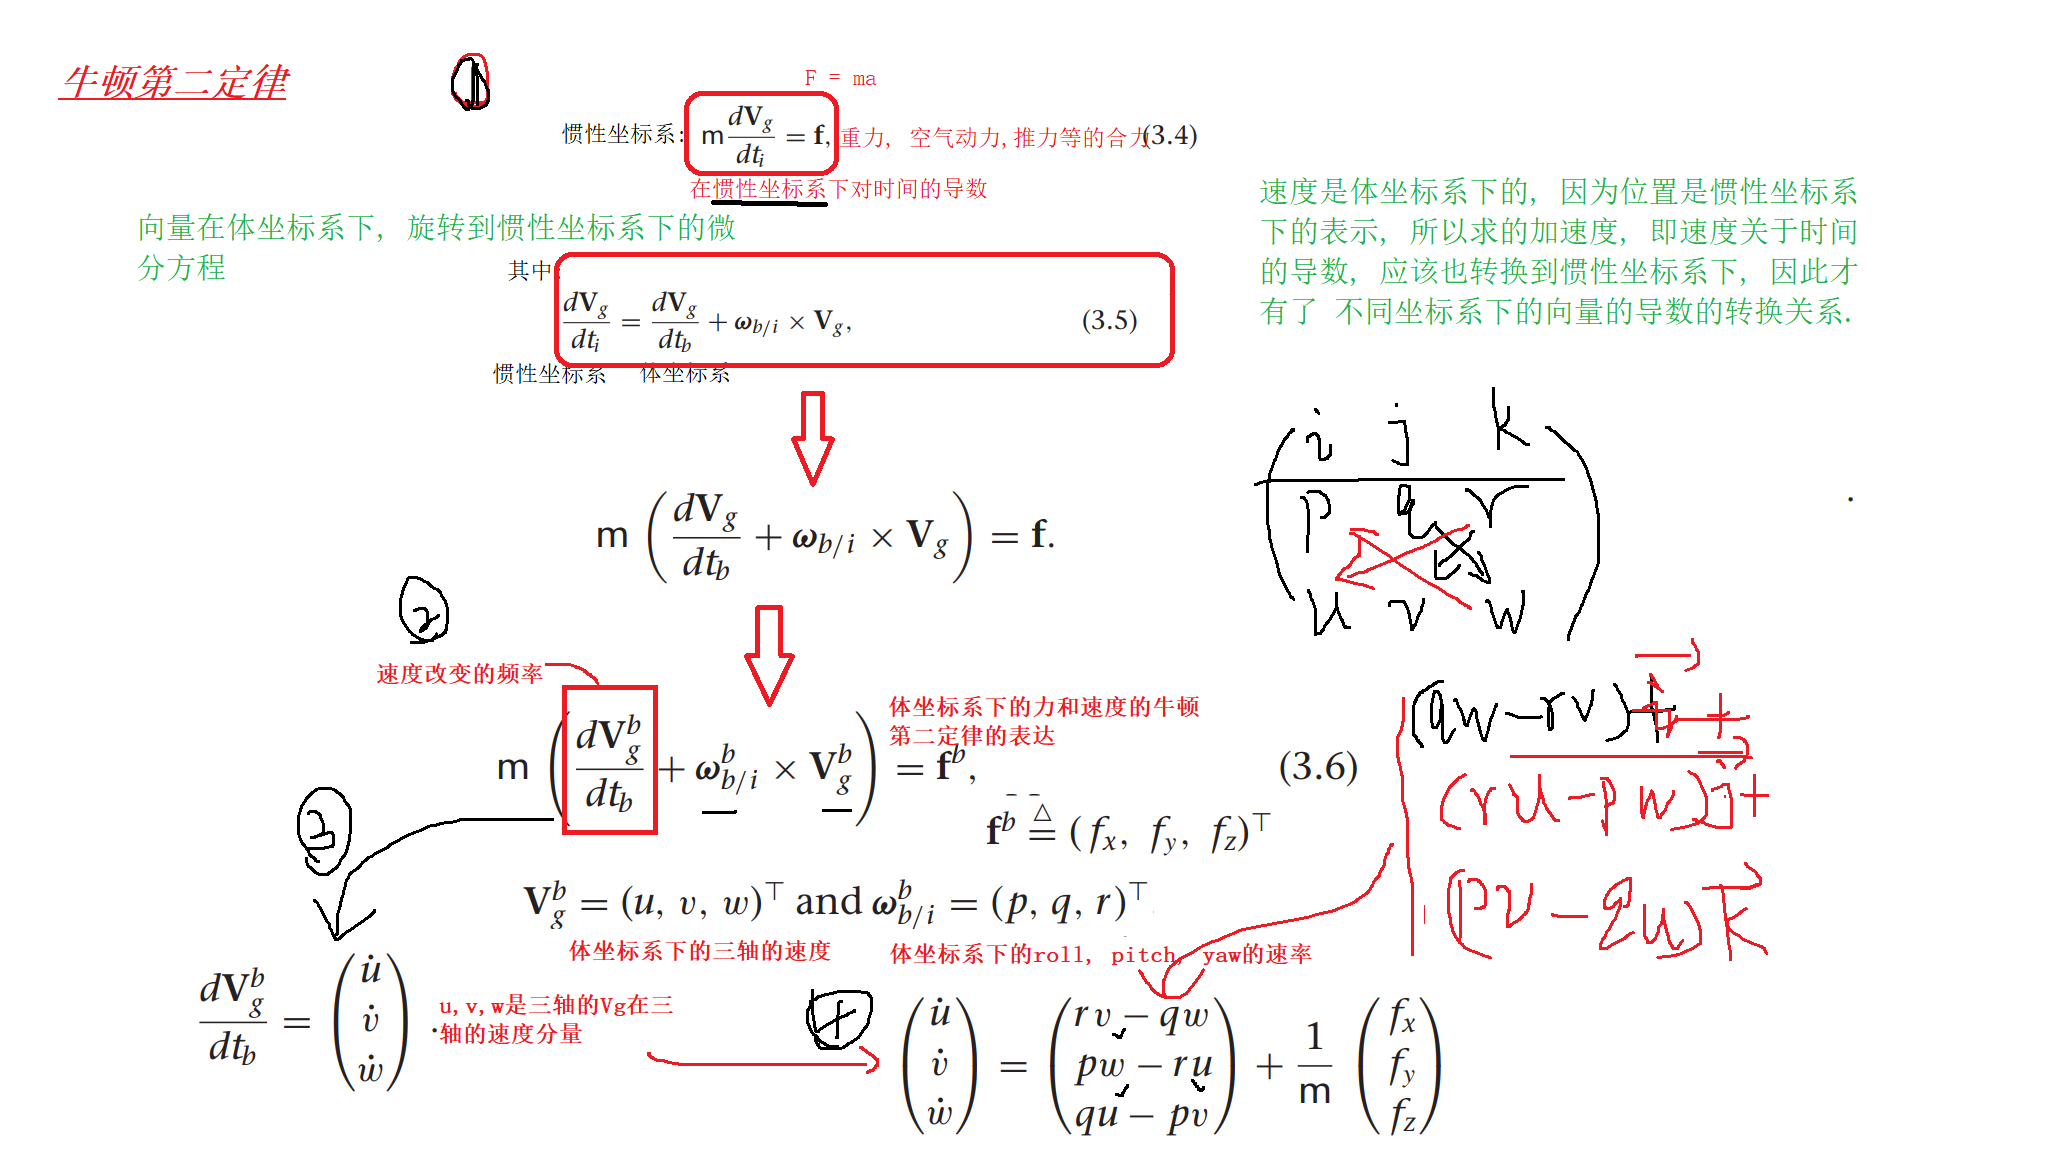
\includegraphics[width=0.8\textwidth]{picture/equ_3.png}
  \caption{牛顿第二运动定律在平移运动下的合并公式}
  \label{equ_3}
\end{figure}
\clearpage
\newpage
\subsection{rotational motion}
针对无人机做旋转运动, 牛顿第二定律作用在物体上面的动力学模型 \ref{equ_5}
\begin{figure}[htpb]
  \centering
  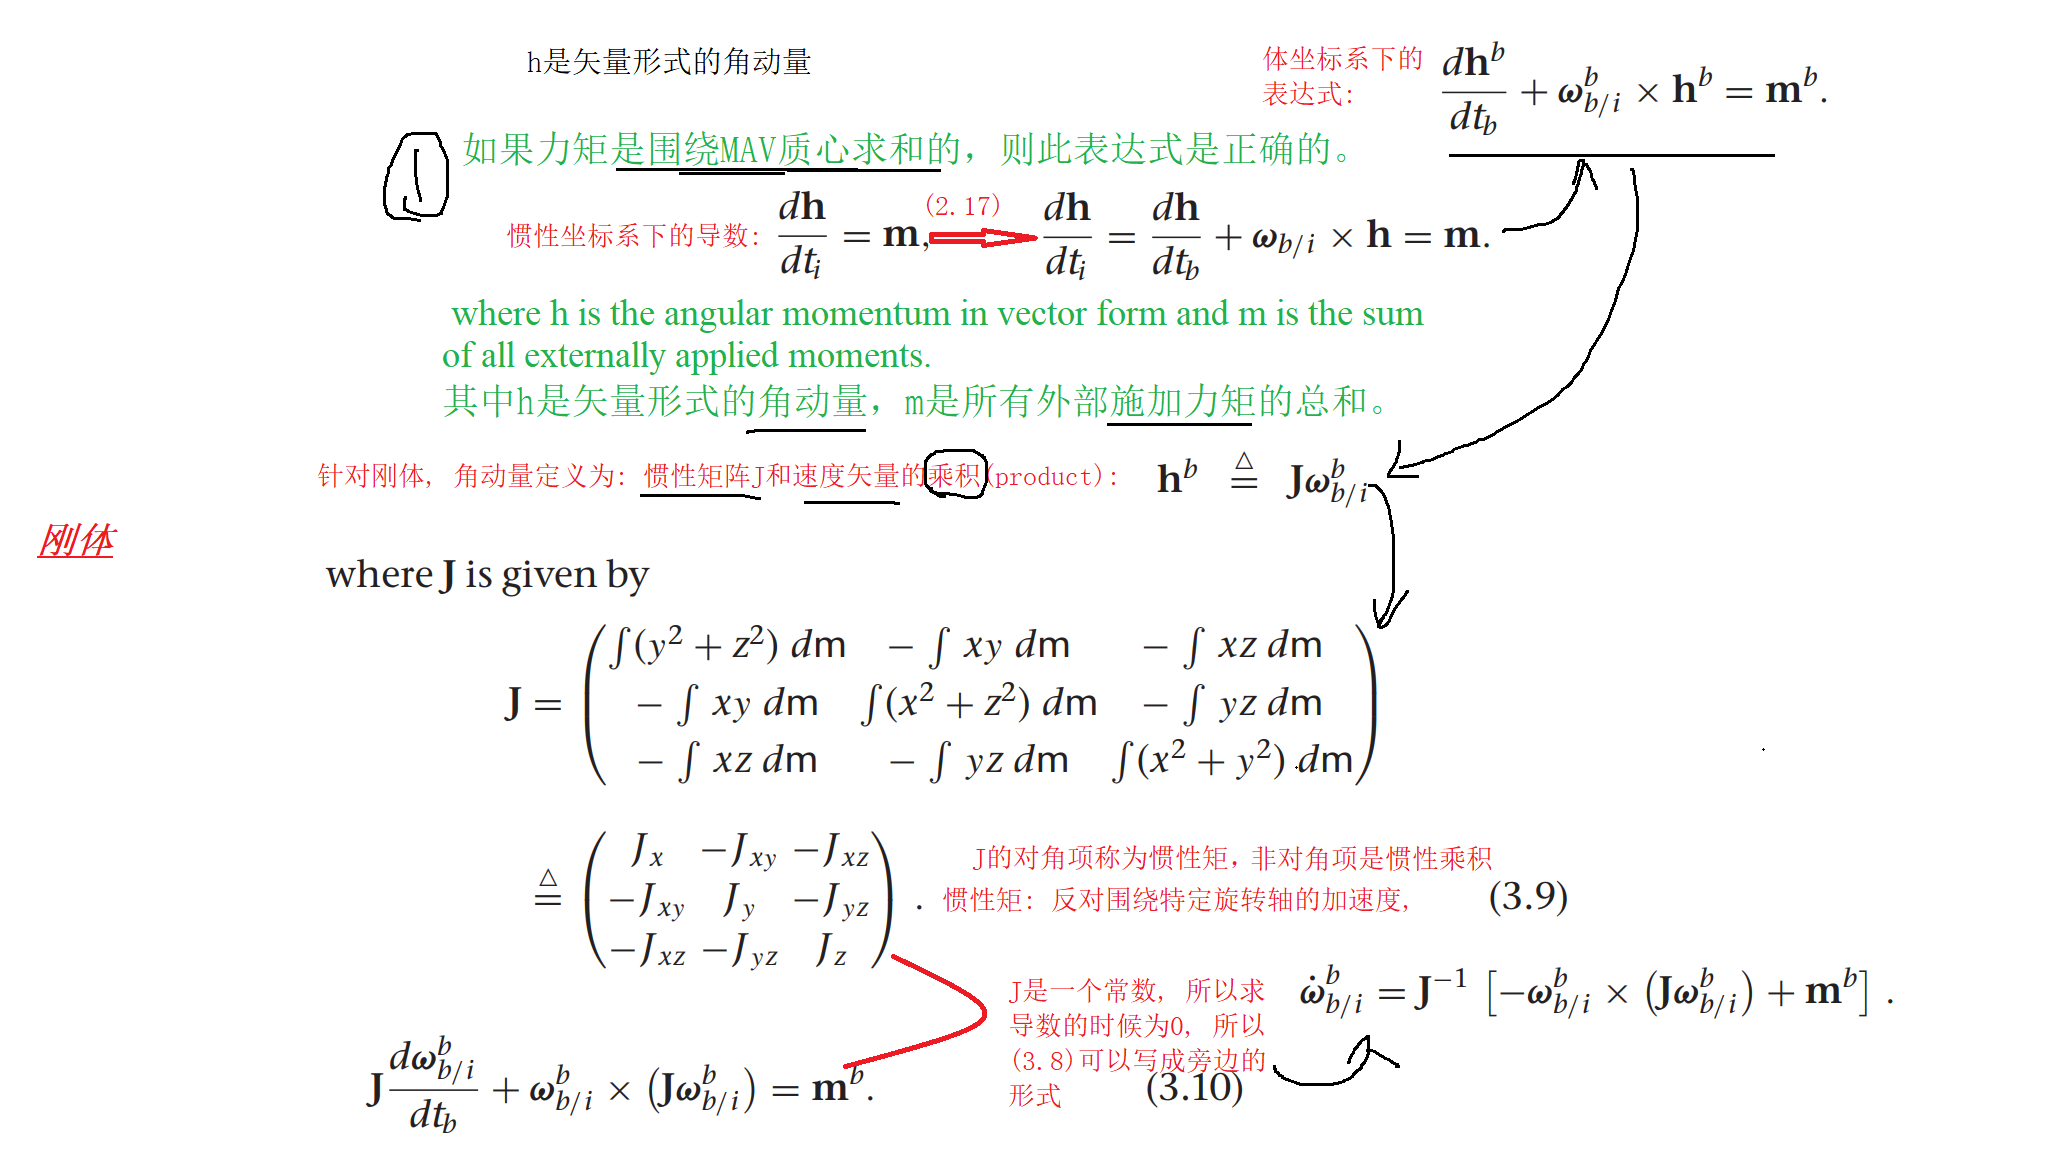
\includegraphics[width=0.8\textwidth]{picture/equ_5.png}
  \caption{牛顿第二运动定律在旋转运动下的合并公式}
  \label{equ_5}
\end{figure}
其中的惯性矩阵\textbf{$J$}的对角项被称为惯性动量, 非对角项是惯性乘积. \par
\textcolor{red}{惯性动量}是飞机的趋势测量, 来抵消无人机关于某一个特定轴的旋转. 比如: $J_{x}$ 是组成飞机的每一个元素的质量的 和 质量元素到体坐标系x的距离的平方($y^{2} + z^{2}$) 的乘积, 再取和. 
$J_{x}$越大, 飞机抵制关于x轴的角加速度越有效. $J_{y}, J_{z}$类似. \par
实际上, 惯性矩阵不能被公式(3.9)进行计算. 而是使用CAD模型从质量的大小计算出来的, 或者也可以通过实验就行测量. 

因为公式(3.19)中的惯性被相对于$i^{b}, j^{b}, k^{b}$轴进行计算的, 且, 这些轴都是固定的, 所以$J$是一个在体坐标系下可见的常数值, 即 $\frac{\mathrm{d} \textbf{J} }{\mathrm{d} t_{b}} = 0$,
所以: 
\begin{equation}
  J \frac{\mathrm{d} \omega_{b / i}^b}{\mathrm{d} t_{b}} + \omega_{b / i} ^ {b} \times (\textbf{J} \omega_{b / i} ^ {b}) = m^{b}
\end{equation}
其中: $\frac{\mathrm{d} \omega_{b / i}^b}{\mathrm{d} t_{b}} $是角速度在体坐标系下对的变化速率
\\ $p, q, r$ 是瞬时$\omega_{b/i}^{b}$在$i^{b}, j^{b}, k^{b}$上的投影. 
所以:
\begin{gather*} % 输入多行公式
  \dot{\omega}_{b/i}^{b} = \frac{\mathrm{d} \omega_{b/i}^{b}}{\mathrm{d} t_{b}} =  \begin{pmatrix}
      \dot{p} \\
      \dot{q} \\
      \dot{r} \\
    \end{pmatrix}
\end{gather*}
\par
飞机通常关于$i^{b}$和$k^{b}$跨越的\textcolor{blue}{平面对称}。在这种情况下,$J_{xy}$ = $J_{yz}$ = 0,这意味着
\begin{gather*}
  J = 
  \begin{pmatrix}
    J_{x} & 0 & -J_{xz} \\
    0 & J_{y} & 0 \\
    -J_{xz} & 0 & J_{z} \\ 
  \end{pmatrix}
\end{gather*}

故, 公式可以推导如下: \ref{equ_6}
\begin{figure}[htpb]
  \centering
  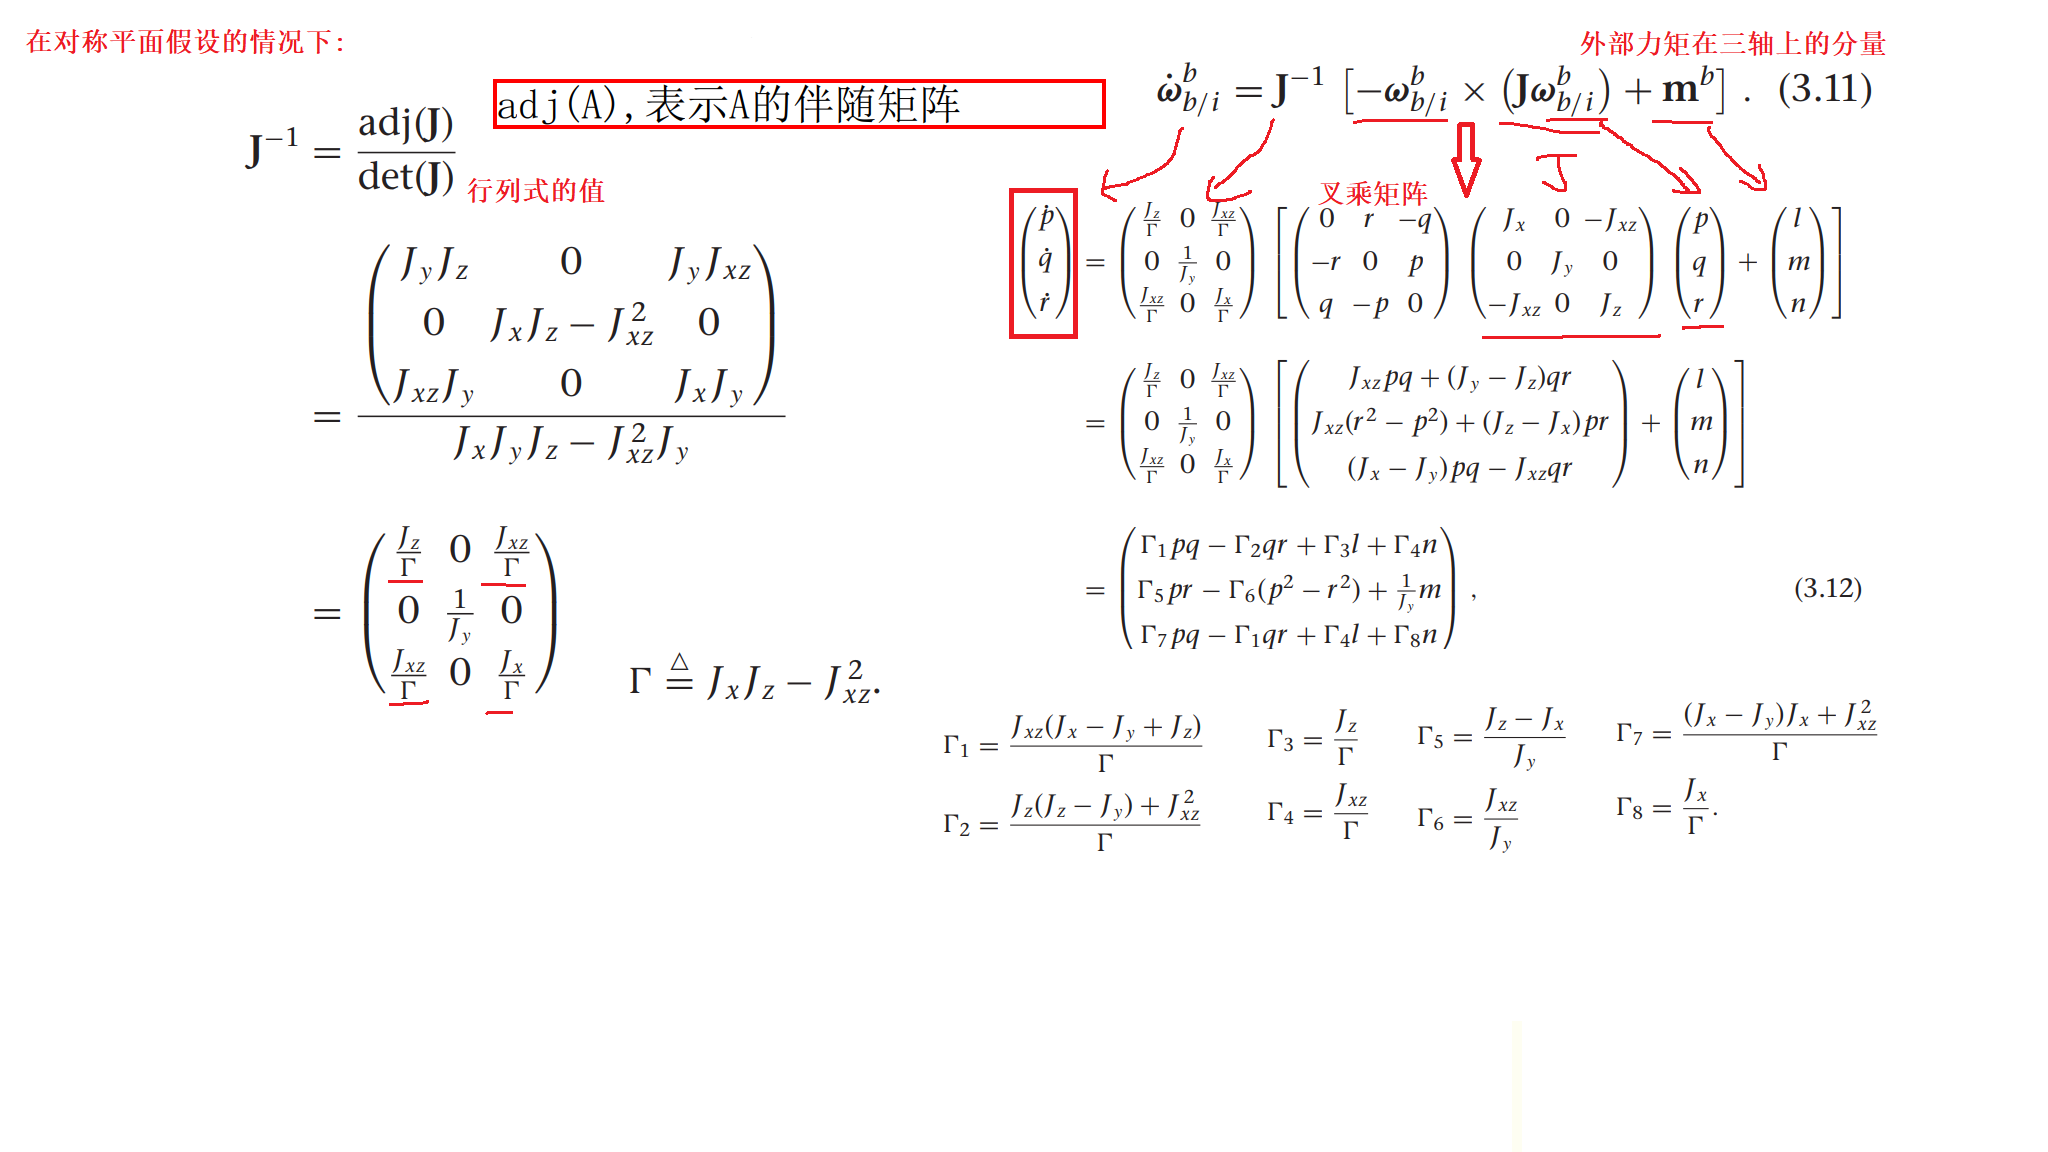
\includegraphics[width=0.8\textwidth]{picture/equ_6.png}
  \caption{公式推导}
  \label{equ_6}
\end{figure}

\section{12个姿态的动力学方程}
本章我们推导出了6个自由度, 和12个姿态动力学模型如\ref{equ_7}所示. 但它们是不完整的, 因为尚未定义外部施加的力和力矩. \par 由重力,空气动力学和推进力而产生的力和力矩的模型将在第4章中得出。
这些模型将会是下面几章分析, 仿真, 和控制设计的基础. 
\begin{figure}[htpb]
  \centering
  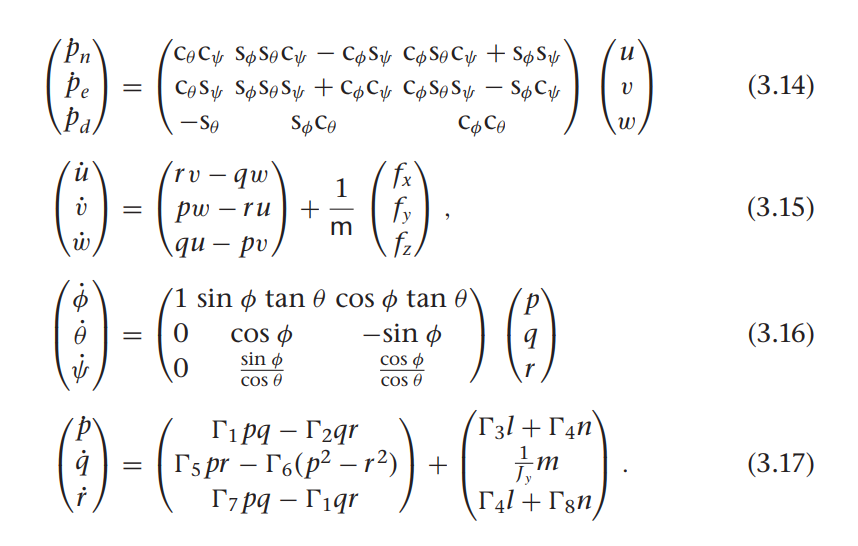
\includegraphics[width=0.8\textwidth]{picture/equ_7.png}
  \caption{动力学方程}
  \label{equ_7}
\end{figure}

\end{document}
